\documentclass{beamer}

\usepackage{ucs}
\usepackage[utf8x]{inputenc}
\usepackage[T1]{fontenc}
\usepackage[english]{babel}

\usepackage[retainorgcmds]{IEEEtrantools}%	IEEEeqnarray

\usepackage{mathabx}%	convolution symbol
\usepackage{multi row}
\usepackage{epstopdf}
\usepackage{listings}
\lstset{
	language=c,
	basicstyle=\footnotesize,
	showtabs=true,
	tabsize=3,
}

%	presentation info
\title{N-Body: Performance profiling}

\author{Miguel Palhas}

\institute[pg19808]{
	Universidade do Minho
}

\date{Braga, December 2011}


%	beamer options
\usetheme{CambridgeUS}


\begin{document}%	begin presentation

\maketitle%	title slide

\begin{frame}
	\frametitle{Index}
	\tableofcontents
\end{frame}

\section{Hardware profile}
\begin{frame}
	\frametitle{Hardware profile: Sources}

	Sources used for a complete profile:
	\begin{description}
		\item[Web] (ark.intel.com, realworldtech.com) For micro architecture information;
		\item[Linux] To print low-level hardware info on BIOS and Kernel;
		\item[Math] For the theorethical values (Peak FP Performance, Peak Mem Bandwith, ...);
		\item[AIDA64] Used to measure cache and main memory latencies.
	\end{description}

\end{frame}

\begin{frame}
	\frametitle{Hardware profile}
	{\small
	\begin{table}[!htp]
		\begin{center}
			\begin{tabular}{|lrl|}
				\hline
				\multicolumn{2}{|l}{\textbf{Manufacturer:}}	&	HP					\\
				\multicolumn{2}{|l}{\textbf{Model:}}		&	Pavilion dv5 1170ep	\\
				\hline
				\hline

				\textbf{Processor:}	& \multicolumn{2}{c|}{\textbf{Core 2 Duo P8600}}	\\
				%\cline{2-3}
				\multicolumn{1}{|c}{\multirow{6}{*}}
					&	Clock frequency			&	2.4 GHz							\\
					&	Peak FP Perf.				&	19.2 GFlop/s				\\
				\hline
				\hline
	
				\textbf{Cache:}	&						&						\\
				\multicolumn{1}{|c}{\multirow{2}{*}{L1}}
					&	Scope			&	Core		\\
					&	Size			&	32KB + 32KB	\\
					&	Associativity	&	8-way		\\
				\hline
				\multicolumn{1}{|c}{\multirow{2}{*}{L2}}
					&	Scope			&	shared		\\
					&	Size			&	3MB			\\
					&	Associativity	&	12-way		\\
				\hline
				\hline
	
				\textbf{Main Memory:}	& \multicolumn{2}{c|}{\textbf{SDRAM DDR2 PC6400}} \\
				\multicolumn{1}{|c}{\multirow{6}{*}}
					&	Frequency		&	800 MHz							\\
					&	Size			&	2x2 GB							\\
					&	Latency			&	81.1 ns 						\\
					&	Peak Bandwith	&	12.8 GB/s						\\
				\hline			
			\end{tabular}
		\end{center}
		\label{tab:profile}
	\end{table}
	}
\end{frame}

\section{Roofline}
\begin{frame}
	\begin{figure}[!htp]
		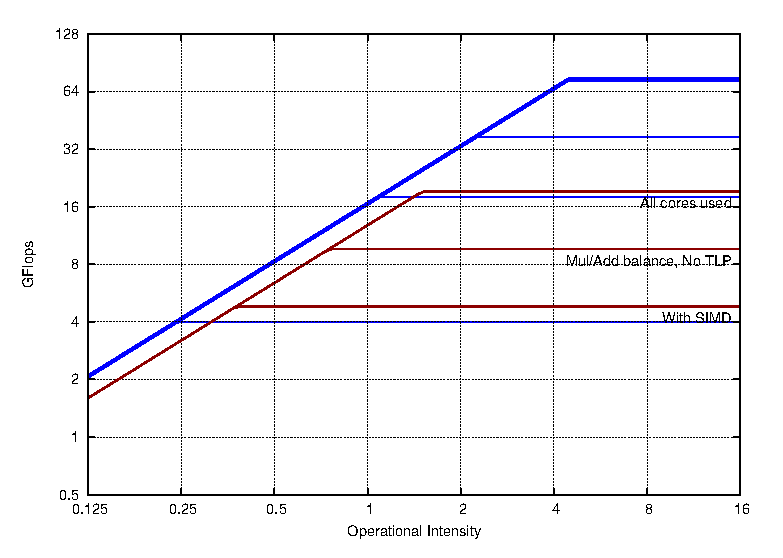
\includegraphics[width=12cm]{images/roofline.eps}
		\label{fig:roofline}
		\caption[Memory benchmark]{Memory benchmark with Aida64 Extreme Edition}
		\end{figure}
\end{frame}

\section{Algorithm}
\begin{frame}%	begin slide
	\frametitle{n-body Algorithm}

	Calculate the movement of a group of objects (e.g. planets) that interact with each other gravitationally

	\begin{IEEEeqnarray}{C}
		{\forall}_{x \in N} \; p_{x}(t + {\Delta}t) = p_{x}(t) + v_{x}(t) + \frac{1}{2}{\Delta}t^{2}a_{x}(t) \nonumber \\
		\; a_{x}(t) = G \sum_{i=1}^{N} \frac{m_{i} | p_{x} - p{i} |}{| p_{x} - p_{i} |} \nonumber \\
	\end{IEEEeqnarray}

	The implementation used runs on $\Theta(N^{2})$ time. However there other more elaborate approaches (not studied here) that can reach $\Theta(N\;log(N))$ \\
\end{frame}%	end slide

\begin{frame}[fragile]
	\frametitle{Square root implementation}

	Standand C sqrt() function is based on Newton's iterative method.
	With $N^{2}$ sqrt() calls, it was impossible to estimate number of instructions executed
	So an alternative function was used (from Quake 3).

	\begin{lstlisting}
	inline double fast_sqrt(const double x) {
	   union { long i; double x; } u;
	   u.x = x;
	   u.i = (((long)1)<<61) + (u.i>>1) - (((long)1)<<51);
	}
	\end{lstlisting}

	About 5 times faster than sqrt(), but very low precision for smaller values.

\end{frame}

\section{Test cases}
\begin{frame}
	\frametitle{Test cases}

	Test cases were selected to fit on the multiple memory levels.
	Each object contains one vector for position, one for velocity, the mass value, and a final vector used for intermediate calculations, resulting in a total of 10 double precision values per objecto (80 Bytes)

	\begin{center}
		\begin{tabular}{|l|l|l|}
			\hline
			\textbf{Test Name}	&	\textbf{Num. Objects (N)}		&	\textbf{Size}	\\
			\hline
			L1\_1				&	64				&	5 KB			\\
			L1\_2				&	128				&	10 KB			\\
			L2\_1				&	8192			&	0.625 MB		\\
			L2\_2				&	16384			&	1.25 MB			\\
			RAM\_1				&	65536			&	5 MB			\\
			RAM\_2				&	131072			&	10 MB			\\
			\hline
		\end{tabular}
	\end{center}
\end{frame}


\subsection{Methodology}
\begin{frame}
	\frametitle{Test Methodology}

	Relevant counters:
	\begin{description}
		\item[PAPI\_TOT\_CYC] Total cycles;
		\item[PAPI\_TOT\_INS] Total instructions
		\item[PAPI\_LD\_INS] Load Instructions
		\item[PAPI\_SR\_INS] Store Instructions
		\item[PAPI\_FML\_INS] Multiply instructions
		\item[PAPI\_FDV\_INS] Division instructions
		\item[PAPI\_VEC\_INS] Vector Instructions
		\item[PAPI\_FP\_OPS] Floating point operations
		\item[PAPI\_L1\_DCA] L1 data cache accesses
		\item[PAPI\_L1\_DCM] L1 data cache misses
		\item[PAPI\_L2\_DCA] L2 data cache accesses
		\item[PAPI\_L2\_DCM] L2 data cache misses
	\end{description}
	Other relevant counters were not available (PAPI\_MEM\_SCY, BUS\_TRANS\_MEM)
\end{frame}

\begin{frame}
	\frametitle{Test Methodology}

	
	\begin{itemize}
		\item Only one core enabled via kernel boot parameters (to avoid process scheduling to a different core)
		\item Graphic environment, network, and other heavy processes disabled
		\item Process niceness set to lowest (or highest priority)
		\item For each Test Size (N), 30 executions of the program (3 for each event, to garantee less than 5\% difference in execution time)
	\end{itemize}

\end{frame}

\section{Results}
\subsection{Memory Accesses}

\begin{frame}[fragile]
	\frametitle{Memory Accesses: Estimated Value}

	Code structure (based on Assembly analysis):
	\\
	\begin{center}
		\begin{lstlisting}
			for(1 to N) {
			   [4 stores, 1 load, 7 instr.]
			   for(1 to N) {
			      [6 stores, 3 loads, 34 instr.]
			   }
			   [3 stores, 6 loads, 26 instr.]
			}
			for(1 to N) {
			   [3 stores, 3 loads, 10 instr.]
			}
		\end{lstlisting}
	\end{center}
\end{frame}

\begin{frame}
	\frametitle{Memory Accesses: Formula}

	Based on the previous code structure, the number of memory accesses can be estimated with:
	$$9N^{2} + 20N$$
	where N is the number of objects being processed.
	\\
	The total estimated number of instruction is given by:
	$$34N^{2} + 43N$$
\end{frame}

\begin{frame}
	\frametitle{Memory Accesses}

	The following table shows the number of memory accesses, by PAPI readings and by estimation from the previous formula

	\begin{table}[!htp]
		\begin{center}
		{\small
			\begin{tabular}{|l|r|r|c|c|}
				
				\hline
				Test	&	PAPI					&	Estimated					&	Est. Error			&	 Accesses/Inst		\\
				\hline
				L1\_1	&	38716					&	38144						&	1.50\%				&	0.27						\\
				L1\_2	&	150588					&	150016						&	0.38\%				&	0.27						\\
				L2\_1	&	604144268				&	604143616					&	0.00\%				&	0.26						\\
				L2\_2	&	2416247656				&	2416246784					&	0.00\%				&	0.26						\\
				RAM\_1	&	38656024690				&	38656016384					&	0.00\%				&	0.26						\\
				RAM\_2	&	154621476174			&	154621444096				&	0.00\%				&	0.26						\\
				\hline
			\end{tabular}
		}
		\end{center}
	\end{table}
\end{frame}

\subsection{Mul/Add balance}
\begin{frame}
	\frametitle{Mult/Add balance}

	There is no counter for Add operations, so it was estimated with
	$$PAPI\_FP\_INS - PAPI\_FML\_INS - PAPI\_FDV\_IN$$

	\begin{table}[!htp]
		\begin{center}
		{\small
			\begin{tabular}{|l|r|r|c|c|}
				
				\hline
				Test	&	FP Mul Inst		&	FP Add Inst		&	Mul/Add balance	\\
				\hline
				L1\_1	&	33555			&	30395			&	90.58\%			\\
				L1\_2	&	133168			&	117874			&	88.52\%			\\
				L2\_1	&	537008683		&	469949801		&	87.51\%			\\
				L2\_2	&	2147782971		&	1879409199		&	87.50\%			\\
				RAM\_1	&	34360620752		&	30066293472		&	87.50\%			\\
				RAM\_2	&	137440660580	&	120261583165	&	87.50\%			\\
				\hline
			\end{tabular}
		}
		\end{center}
	\end{table}
\end{frame}

\subsection{CPI}
\begin{frame}
	\frametitle{CPI}

	Calculated based on FPI\_TOT\_INS and FPI\_TOT\_CYC

	\begin{table}[!htp]
		\begin{center}
		{\small
			\begin{tabular}{|l|r|r|c|c|}
				
				\hline
				Test	&	Instructions	&	Cycles			&	CPI		&	IPC		\\
				\hline
				L1\_1	&	143317			&	135750			&	0.95	&	1.06	\\
				L1\_2	&	563861			&	472027			&	0.84	&	1.19	\\
				L2\_1	&	2282055015		&	1686732377		&	0.74	&	1.35	\\
				L2\_2	&	9127511619		&	6775496328		&	0.74	&	1.35	\\
				RAM\_1	&	146031715237	&	171062387955	&	1.17	&	0.85	\\
				RAM\_2	&	584121221418	&	687083107943	&	1.18	&	0.85	\\
				\hline
			\end{tabular}
		}
		\end{center}
	\end{table}
\end{frame}

\subsection{Miss rates}
\begin{frame}
	\frametitle{Miss rates}% %miss / case size

	Based on the counters that give total accesses and misses to both L1 and L2 cache levels

	\begin{table}[!htp]
		\begin{center}
		{\small
			\begin{tabular}{|l|r|r|c|c|}
				
				\hline
				Test	&	L1 Accesses		&	L1 Miss \%	&	L2 Accesses		&	L2 Miss \%	\\
				\hline
				L1\_1	&	50287			&	0.20\%		&	290				&	33.79\%		\\
				L1\_2	&	194416			&	0.10\%		&	476				&	34.03\%		\\
				L2\_1	&	750943668		&	11.18\%		&	219910694		&	0.01\%		\\
				L2\_2	&	3007631681		&	11.18\%		&	882123490		&	0.01\%		\\
				RAM\_1	&	48304577585		&	11.14\%		&	10917610760		&	46.85\%		\\
				RAM\_2	&	194497858380	&	11.06\%		&	42817380648		&	50.25\%		\\
				\hline
			\end{tabular}
		}
		\end{center}
	\end{table}
\end{frame}

\subsection{Operational Intensity}
\begin{frame}
	\frametitle{Operational Intensity}

	Attempted to estimate Bytes read from RAM with L2\_MISSES * 64, assuming that every miss will issue a new cache line read from RAM (64 Bytes)
	However:
	\begin{itemize}
		\item L2 counters are derived (maybe not reliable?)
		\item \#L1 misses <> \#L2 accesses. So we can also assume that \#L2 misses <> \#RAM accesses, making the previous formula wrong
	\end{itemize}

	\begin{table}[!htp]
		\begin{center}
		{\small
			\begin{tabular}{|l|r|r|r|r|}
				\hline
				Test	&	L2 Misses		&	Bytes from RAM		&	FP Inst.		&	Op. Intensity	\\
				\hline
				L1\_1	&	98				&	6272				&	68110			&	10.86			\\
				L1\_2	&	162				&	10368				&	267551			&	25.81			\\
				L2\_1	&	11434			&	731776				&	1074075321		&	1,467.77		\\
				L2\_2	&	103001			&	6592064				&	4295643580		&	651.64			\\
				RAM\_1	&	5114423222		&	0.3e+11 (0.3 TB)	&	68721939721		&	0.21			\\
				RAM\_2	&	21517065599		&	1.3e+12 (1.3 TB)	&	274882221251	&	0.20			\\
				\hline
			\end{tabular}
		}
		\end{center}
	\end{table}

	Actually, 1.3 TB is near the calculated value that should be read from RAM if there was no cache in between.\\
	$$N^{2} \times 80 Bytes = 131072^{2} \times 80 Bytes = 1.25 TB$$

	So given the 50\% Miss Rate from L2 Cache, it was expected that the number of Bytes read from RAM was around half, or 0.65 TB, which is not the case.\\

		For L2 Tests, the very high Operational Intensity is due to an increase of the data set (L2\_1 is 64 times bigger than L1\_2) but still with enough size to fit in L2 cache, which lowers the number of reads from RAM.

\end{frame}

\section{Conclusion}
\begin{frame}
	\frametitle{Conclusion}
	\begin{itemize}
		\item Some difficulties measuring memory ceilings. The Roofline paper used a custom Stream benchmark, and provided no theorethical way to estimate those values;
		\item PAPI counters may sometimes differ from what is expected, especially when measuring memory traffic;
		\item TLP was not explored, and it would certainly prove beneficial and easili implemented for this particular algorithm;
	\end{itemize}
\end{frame}

\section{References}
\begin{frame}
	\frametitle{References}

	\begin{itemize}
		\item Intel 64 and IA-32 Architectures Optimization Reference Manual
		\item PAPI Documentation (http://icl.cs.utk.edu/papi/)
		\item Best Square Root Method, Precision VS Speed (http://www.codeproject.com/KB/cpp/Sqrt\_Prec\_VS\_Speed.aspx)
		\item OpenCL N-Body Simulation (http://www.browndeertechnology.com/docs/BDT\_OpenCL\_Tutorial\_NBody-rev3.html)
	\end{itemize}
\end{frame}

\section{Questions}
\begin{frame}
	\titlepage
	\begin{center}
		\Huge\bfseries
		- ? -
	\end{center}
\end{frame}

\end{document}%	end presentation
